\chapter{The Compact Muon Solenoid Experiment at the Large Hadron Collider}
\label{ch:detector}

%OLD
%The particles we, and every stable matter we know consist of are protons, neutrons and electrons. The first two named consists of %up and down quarks. To investigate all of the particles of the standard model and all their interactions with each others, %physisists had to develope experiment with ever higher energeries and precision.
%
%Particle accelerator experiments have a great story of sucess in the investigation of the physical laws. With these machines it %was able to prove the existence of different elementary particles of the standart model. Just a few years ago, in 2012, the last %missing part of the standard model, the higgs boson, was observed \cite{CMS_higgs_1207} \cite{ATLAS_higgs_1207} at the Large %Hadron Collider (LHC) with the Compact Muon Solenoid (CMS) and A Toroidal LHC ApparatuS (ATLAS) experiments. The following %section gives a short description of the LHC, the second section of this chapter will biefly explain the CMS experiment.

Particle accelerator experiments have a great history of success in the investigation of physical laws. With these machines, it was possible to prove the existence of different elementary particles of the standard model, for instance, the top quark \cite{tdiscovery}. Particle accelerators make use of the electric charge of particles to accelerate them to velocities close to the speed of light. In a circular collider, particles are moving in circles in opposite directions and are forced to head-on collisions. These collisions release a high amount of energy and because of the laws of physics, heavy particles are produced that are highly unstable and decay after a short time. Detectors are used to measure the properties of these particles directly or indirectly.\\

This chapter gives a brief overview of the collider and detector system that has produced and measured the events used in this work. 

\section{The Large Hadron Collider}
The Large Hadron Collider (LHC) \cite{lhcguide,lhcweb} is a circular collider located at the European Organization for Nuclear Research (CERN) in the region of Geneva. With a circumference of 27\,km, it is the world's largest and most powerful particle accelerator and lies in a tunnel about 100 m beneath the earth. The LHC is used to accelerate protons, xenon ions and lead ions. These particles undergo several steps of creation and pre-accelecation before they are injected into the LHC. An illustration of the system is shown in figure~\ref{fig:ch_2_cernacccompl}.\\

\begin{figure}
\centering
\includegraphics[width=0.75\textwidth]{assets/CERN_accelerator_complex.png}
\caption[CERN Accelerator Complex]{\textbf{The CERN accelerator complex.} The figure shows several accelerator facilities at CERN. The protons that end up in the LHC are obtained from hydrogen atoms and are first accelerated with the \textcolor{LINAC2}{LINAC2} accelerator to 50\,MeV. Next, they are injected into the \textcolor{LINAC2}{Booster} accelerator and are accelerated to 1.4\,GeV. It follows the acceleration in the \textcolor{PS}{Proton Synchrotron (PS)} to 25\,GeV and in the \textcolor{SPS}{Super Proton Synchrotron (SPS)} to 450\,GeV. Finally, the protons are injected into the \textcolor{LHC}{LHC} in both directions. From there they reach a final energy of 6.5\,TeV within 20 minutes. In addition, the four main detectors at the LHC are shown. Source: \cite{cernacccompl}}
\label{fig:ch_2_cernacccompl}
\end{figure}

The LHC consists of two beam pipes, allowing the acceleration of protons in opposite directions. In this setup, for head-on collisions with equal beam energies, the center-of-mass energy is twice the beam energy $E$:
\begin{equation}
\sqrt{s} = 2 \cdot E \quad .
\end{equation}
In 2010, the first collisions with a beam energy of 3.5\,TeV started. In 2012, the center-of-mass energy was increased to $\sqrt{s} = 8$\,TeV. From 2013 to 2015, the LHC was shut down for maintenance. After this, Run 2 started in 2015 with $\sqrt{s} = 13$\,TeV. After a shutdown in 2018, the LHC is planned to run at $\sqrt{s} = 14$\,TeV in 2021 for Run 3. \\

The protons in the beam are packed in up to 2808 bunches, each bunch consists of about $1.2 \cdot 10^{11}$ protons. For each beam, eight superconducting cavities, cooled down to 4.5\,K, generate an electromagnetic potential with a frequency of 400\,MHz to accelerate and tighten the bunches. Each of the cavities is delivering an accelerating field of 5\,MV/m. To avoid collisions with gas molecules during operation, the beam pipes have a ultrahigh vacuum pressure of $10^{-13}$\,atm. Dipole magnets with a magnetic field strength of up to 7.74\,T each, force the particle beam to stay on the circular path. Quadrupole magnets and magnets of higher order are used to focus the beam. To keep the magnets in superconducting state, superfluid helium is used to cool them down to 1.9\,K. \\

Besides the center-of-mass energy, the luminosity is another important quantity for particle accelerators. The luminosity $L$ determines the event rate and therefore, a high luminosity is desired: 

\begin{equation}
\frac{\mathrm{d}N}{\mathrm{d}t} = \sigma L \quad ,
\end{equation}\label{eq:ch_2_dN}

where $N$ is the number of events and $\sigma$ is the cross section, given by the physical laws described in chapter \ref{ch:theory}. The luminosity depends on the properties of the particle accelerator:

\begin{equation}
L = \frac{n  N_1  N_2  f}{A} \quad .
\end{equation}\label{eq:ch_2_L}

Here, $n$ is the total number of bunches in the collider, $N_1$ and $N_2$ are the number of particles in the colliding bunches, $f$ is the circulating frequency for one single bunch and $A$ is the cross-sectional area. As the luminosity is inversely proportional to the area, the beam must be focused as much as possible to reach a high luminosity. The total number of events can be derived by integrating equation \ref{eq:ch_2_dN} over time to

\begin{equation}
N = \sigma \int L \textrm{d}t = \sigma \mathcal{L} \quad ,
\end{equation}

with the integrated luminosity $\mathcal{L}$. In 2016, a peak luminosity of $1.5 \cdot 10^{34}\,\textrm{cm}^{-2}\textrm{s}^{-1}$ was reached with an integrated luminosity of $41\,\textrm{fb}^{-1}$ ($1\,\textrm{b} = 10^{-24}\,\textrm{cm}^2$) for the total year \cite{lhclumi2016}. After Run 3 at the LHC, a high luminosity upgrade is planned in which the luminosity will be increased to $5 \cdot 10^{34}\,\textrm{cm}^{-2}\textrm{s}^{-1}$.\\

There are four interaction points at the LHC. At each point, one detector is located. One is for the ALICE experiment that studies collisions of lead ions. Another one is for the LHCb experiment, which is designed for the studies of b hadron physics. The ATLAS and the CMS experiments are general-purpose experiments, measuring the standard model particles and searching for new elementary particles.


\section{The Compact Muon Solenoid Detector}
The construction of the Compact Muon Solenoid (CMS) detector \cite{CMSDesignReport} was motivated by the search for the Higgs boson and the search for physics beyond the standard model. The former one has already been found \cite{ATLAS_higgs_1207,CMS_higgs_1207}, but the search for alternative theories like supersymmetry or extra dimensions is still ongoing. Besides of these two big tasks, the CMS detector is used for several other studies, like the measurement of the couplings of different particles \cite{tHq}.
In order to achieve these goals, the detector is required to measure the properties of all particles with best possible precision. A sketch of a slice of the CMS detector with its different sub-detectors is shown in figure \ref{fig:ch_2_cmsslice}. To store only the interesting events and reduce the amount of data to an amount that can be stored for further analyses, a filter system, the so called trigger system, is applied. In this section, the sub-detectors and the trigger system are briefly described. At the beginning the coordinate system used within the CMS detector is introduced.

\begin{figure}
\centering
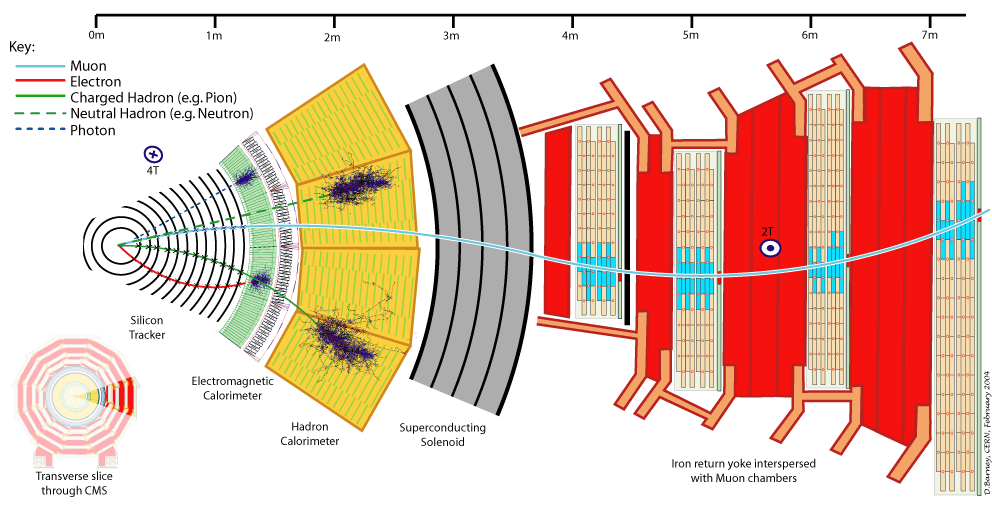
\includegraphics[width=0.75\textwidth]{assets/CMS_Slice.png}
\caption[CMS Detector Slice]{\textbf{Slice of the CMS detector.} The scheme shows the different detector systems as well as the tracks and the interactions of different particles with the detector. Source: \cite{cmsslice}}
\label{fig:ch_2_cmsslice}
\end{figure}

\subsection*{Coordinate System}
The origin of the coordinate system is chosen to be the intended collision point. The $z$ axis points in beam direction. The $x$ axis lies in the plane of the collider ring and points to its center. The $y$ axis points vertically upwards. The azimuthal angle $\phi$ is defined as the angle in the $x$-$y$ plane measured from the $x$-axis. The radial distance is $r = \sqrt{x^2 + y^2}$. The polar angle $\theta$ is measured from the $z$ axis. Another important quantity is the rapidity, which is a measure for the velocity of a particle and defined as
\begin{equation}
y = \textrm{artanh}\left(\frac{v}{c}\right) \quad ,
\end{equation}
where $v$ is the velocity of the particle and $c$ is the speed of light. $y$ is in contrast to $v$ unlimited and can take values in the range of $-\infty$ to $\infty$, further one can just add two rapidities together instead of using the relativistic valocity-addition formula. The pseudorapidity $\eta$ is a frequently used quantity in particle physics, in the relativistic approximation, $\eta$ is equal to $y$ and given by the equation
\begin{equation}
\eta = -\ln\left[\tan\left(\frac{\theta}{2}\right)\right] \quad ,
\end{equation}
which is used to denote the angle between a vector and the $z$ axis. A value of $\eta = 0$ is equal to $\theta = 90^{\circ}$; an angle of $\theta = 0^{\circ}$ equals $\eta = \infty$. The pseudorapidity is preferred over $\theta$ since the number of produced particles per $\eta$-interval is constant and the difference between two particles $\Delta\eta$ is invariant under lorentz boosts in $z$ direction. The momentum and energy of the initial partons is not determined in a hadron collider. Because of this, mainly the quantities transverse to the beam axis are of interest. These quantities, the transverse momentum \pt and the transverse energy \Et are invariant under lorentz boosts in $z$ direction. They are defined as 

\begin{equation}
\pt = \sqrt{p_{x}^2 + p_{y}^2} \quad \textrm{and} \quad \Et = \sqrt{E_x^2 + E_y^2} \quad .
\end{equation} 

Due to momentum conservation, the transverse momenta of all final particles sum up to zero. In the measurement there is always a missing amount of transverse momentum caused by gaps in the detector and neutrinos, which are not detectable within the CMS detector. The missing amount of transverse momentum is denoted as $p_\textrm{T}^{\textrm{miss}}$. 

\subsection*{Silicon Tracker}
Immediately after the collision, heavy objects are formed which decay after a short time and distance. The innermost part of the detector is of highest importance to reconstruct these objects and has to fulfill several requirements. First, a precise measurement of trajectories of charged particles is necessary to identify primary and secondary vertices. This also allows a momentum measurement as the full tracker is inside the superconducting solenoid, which produces a homogeneous magnetic field of 4\,T. Next, at each bunch crossing, about 1000 particles on average are created and travel through the detector. To distinguish these particles from each other and to assign the trajectories to the corresponding vertices, a high granularity is needed. Further, the time between two bunch crossings is about 25\,ns, therefore the response time and the cooling down period has to be short. Last, the detector components have to be resilient against this high amount of radiation.\\

To fulfill these requirements, silicon technology is used for the whole tracker system \cite{tracker}. When charged particles travel through these materials, electron-hole pairs are produced, which in turn generate an electric current in the read-out electronics. In the innermost part from $r=4.4$\,cm to 10.2\,cm, three barrel layers of pixel detectors are surrounding the beam axis. Each pixel detector has a size of 100\,$\times$\,150\,$\upmu \textrm{m}^2$. With this design, the desired impact parameter resolution is achieved. The pixel detectors are surrounded by ten layers of silicon micro-strip detectors up to a radius of 1.1\,m. As the particle flow decreases with the radius, larger detector elements can be used. This also reduces the amount of read-out electronics. The inner micro strip detectors have a size of 10\,$\textrm{cm}$\,$\times$\,80\,$\upmu \textrm{m}$, whereas the size of the outer ones is 25\,$\textrm{cm}$\,$\times$\,180\,$\upmu \textrm{m}$. 
At the endcaps, two disks of pixel detectors, three smaller and nine larger discs of strip detectors are installed. This allows a reconstruction of charged particle tracks up to $|\eta| < 2.5$. In total, the silicon tracker has a length of 5.8\,m with a diameter of 2.5\,m. At each bunch crossing, the occupancy of the detectors is at about 2-3\% for the inner micro strip detectors and 1\% or lower for the other ones. The track resolutions for charged particles of $1\,\GeV < \pt < 10\,\GeV$ and $|\eta| < 1.4$ are typically 1.5\% in \pt, 25--90 \mum in the transverse and 45--150 \mum in the longitudinal impact parameter \cite{trackerPerformance}.


\subsection*{Electromagnetic Calorimeter}
The electromagnetic calorimeter (ECAL) \cite{ECAL} surrounds the silicon tracker system hermetically and measures the energy of electrons, positrons and photons. Other electromagnetically interacting particles leave tracks but are not fully absorbed in the ECAL. The ECAL consists of several elements, the pseudorapidity interval up to $|\eta|<1.48$ is covered bu the barrel part while the endcap has a coverage of $1.48 < |\eta| < 3 $. The ECAL consists of homogeneous lead tungstate ($\textrm{PbWO}_4$) crystals which is the absorber and scintillator material at the same time. When electromagnetically interacting particles propagate through it, they produce photons through bremsstrahlung, which in turn create electron-positron pairs through pair production. An electromagnetic shower emerges. When the energy of the electrons drops to a critical amount, they mainly excite the atoms, which emit photons with characteristic wavelengths between 360\,\nm to 570\,\nm. This process is called scintillation. The photons are then measured with photomultipliers. The number of photons is proportional to the deposited energy of the particle. The radiation length of $\textrm{PbWO}_4$ is $X_0=0.89$\,cm. This means that after this distance, the energy of an electron or positron is reduced on average by the factor of 1/e. Moreover a photon has an average free path length of $9/7$ $X_0$ before it undergoes a process of pair production. The thickness of the ECAL with 23\,cm is equivalent to 25.8 $X_0$, therefore all electrons, positrons and photons are absorbed completely. \\

The ECAL was designed to measure the H $\rightarrow \upgamma \upgamma$ decay as precise as possible. Therefore, it provides a good energy resolution. To identify the background in this decay channel, a preshower detector is installed between the tracker and the ECAL. This element helps to identify neutral pions that decay into two photons; it also improves the position determination of electrons, positrons and photons. 

\subsection*{Hadron Calorimeter}
Hadrons propagate through the ECAL losing only a small fraction of their energy. Therefore, a hadron calorimeter (HCAL) \cite{HCAL} surrounds the ECAL, which absorbs all hadrons and measures their energy. The HCAL is important for measuring the properties of hadron jets as well as the total energy of the collisions and the resulting missing transverse energy. Several elements allow to measure forward jets up to $|\eta| = 5.2$. \\

The HCAL is a sampling calorimeter which exists of alternating absorbing layers and scintillating layers. The absorbing layer consists of brass and has a nuclear interaction length of $\lambda_\textrm{I} = $16.42\,cm. This is the mean distance for a hadronic particle after which it undergoes an inelastic nuclear interaction. Similar to the ECAL, a chain reaction starts and a hadronic shower emerges. As the HCAL is located inside the solenoid, its size is limited. The total absorber material of ECAL and HCAL makes up less than 7 $\lambda_\textrm{I}$. For hadrons that are not fully absorbed, an additional outer hadron calorimeter is installed outside the solenoid.
For the scintillating layers, plastic is used. When the hadronic shower hits these layers, the scintillator material gets excited and photons with characteristic wavelengths are emitted. They are guided through optical cables and measured by photodiodes.

\subsection*{Muon Detector}
The muon detector \cite{MuonChamber} is the outermost part of the CMS detector and covers the pseudorapidity interval of $|\eta| < 2.4$ without any gaps. The only particles that reach this part of the detector are neutrinos, which cannot be detected directly with the CMS detector, and muons. Muons have a high mass and are often high energetic. Because of this, they lose only small parts of their energy by propagating through the inner parts and are usually not fully absorbed in the muon detector. Muon identification and position determination is done with gaseous detectors. As they pass through these detectors, muons are ionizing the gas atoms. The resulting electrons and ions can then be measured as an electric current. The muon system consists of an iron return joke to guide the magnetic field lines of the solenoid through this part of the detector. This creates a magnetic field of 2\,T. As a consequence, muons travel a circular path. The momentum can then be determined by measuring the radius of its track. 

\subsection*{Trigger System}
The LHC has a bunch crossing rate of about 40\,MHz at each interaction point. This huge amount of data makes it impossible to store every event. Since interesting processes typically have low rates, it is sufficient for most analyses to store only a small fraction of promising events. To perform this data reduction, a trigger system \cite{TriggerDesignRep} consisting of two filtering steps is used at the CMS detector.\\

 The first filter is called the Level-1 (L1) trigger and is realized by hardware electronics. It decides in a few $\upmu$s whether it is worth keeping an event. In this short time, only a part of the information from the calorimeters and the muon chamber can be used. The trigger checks if the information is consistent with a physics object like an electron or a muon. This procedure reduces the event rate to less than 100\,MHz. \\

The second filter step is done by the High-Level Trigger (HLT). The HLT is realized with software tools where complex calculations and a more precise reconstruction can be done. In addition, the information of the tracking system is now included. This trigger reduces the event rate further to less than 1.5\,KHz. These events are then stored offline for more detailed analyses. 
